\documentclass[tikz,border=10pt]{standalone}
\usepackage{mathabx}
\usetikzlibrary{backgrounds}
\usepackage{newunicodechar}
\newunicodechar{♮}{$\natural$}
\newunicodechar{♭}{$\flat$}
\newunicodechar{♯}{$\sharp$}
\newunicodechar{➚}{$\nearrow$}
\newunicodechar{➘}{$\searrow$}
\newunicodechar{ʼ}{'}
\newunicodechar{Ȧ}{\stackon[0.8pt]{A}{.}}
\newunicodechar{Ḃ}{\stackon[0.8pt]{B}{.}}
\newunicodechar{Ċ}{\stackon[0.8pt]{C}{.}}
\newunicodechar{Ḋ}{\stackon[0.8pt]{D}{.}}
\newunicodechar{Ė}{\stackon[0.8pt]{E}{.}}
\newunicodechar{Ḟ}{\stackon[0.8pt]{F}{.}}
\newunicodechar{Ġ}{\stackon[0.8pt]{G}{.}}


\def\centerarc[#1](#2)(#3:#4:#5);%
{
  \draw[#1]([shift=(#3:#5)]#2) arc (#3:#4:#5);
}


\begin{document}
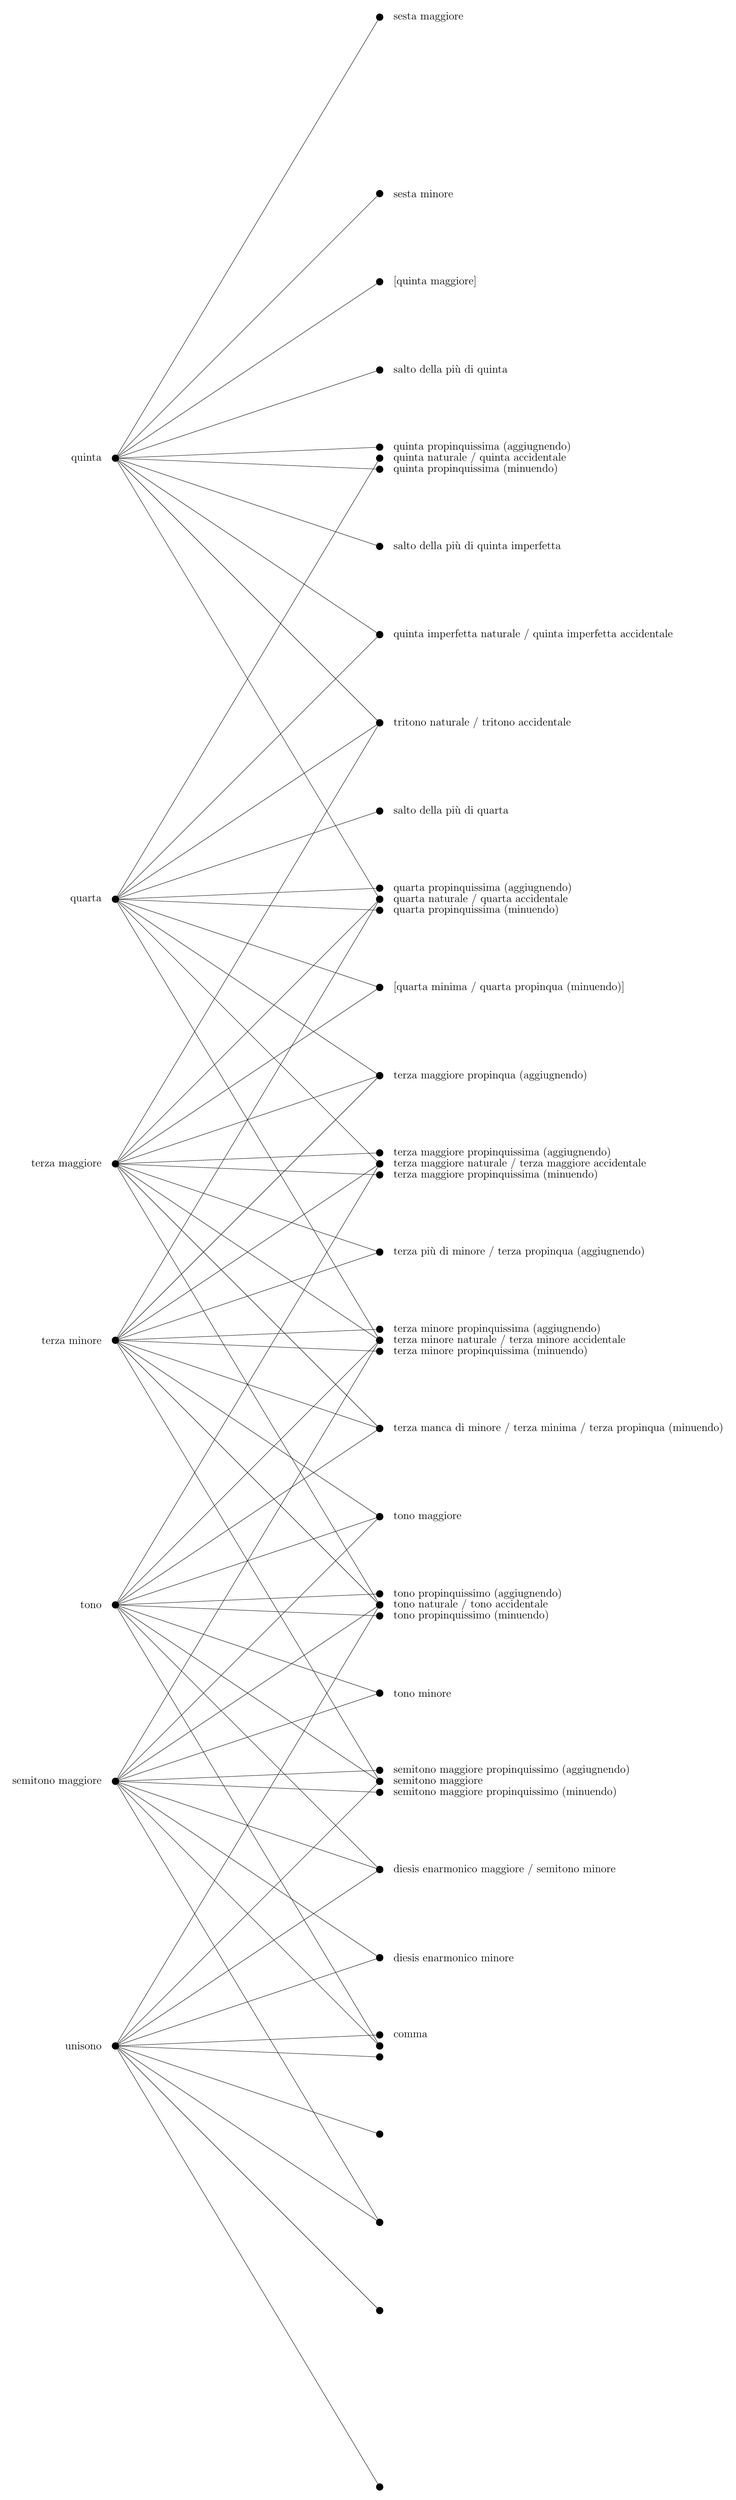
\begin{tikzpicture}

\draw (1.6666666,0.0) -- (11.666667,0.41666666);
\draw (1.6666666,0.0) -- (11.666667,-0.41666666);
\draw (1.6666666,0.0) -- (11.666667,3.3333333);
\draw (1.6666666,0.0) -- (11.666667,-3.3333333);
\draw (1.6666666,0.0) -- (11.666667,6.6666665);
\draw (1.6666666,0.0) -- (11.666667,-6.6666665);
\draw (1.6666666,0.0) -- (11.666667,10.0);
\draw (1.6666666,0.0) -- (11.666667,-10.0);
\draw (1.6666666,0.0) -- (11.666667,16.666668);
\draw (1.6666666,0.0) -- (11.666667,-16.666668);
\draw (1.6666666,10.0) -- (11.666667,10.416667);
\draw (1.6666666,10.0) -- (11.666667,9.583334);
\draw (1.6666666,10.0) -- (11.666667,13.333333);
\draw (1.6666666,10.0) -- (11.666667,6.6666665);
\draw (1.6666666,10.0) -- (11.666667,16.666668);
\draw (1.6666666,10.0) -- (11.666667,3.3333333);
\draw (1.6666666,10.0) -- (11.666667,20.0);
\draw (1.6666666,10.0) -- (11.666667,0.0);
\draw (1.6666666,10.0) -- (11.666667,26.666666);
\draw (1.6666666,10.0) -- (11.666667,-6.6666665);
\draw (1.6666666,16.666668) -- (11.666667,17.083334);
\draw (1.6666666,16.666668) -- (11.666667,16.25);
\draw (1.6666666,16.666668) -- (11.666667,20.0);
\draw (1.6666666,16.666668) -- (11.666667,13.333333);
\draw (1.6666666,16.666668) -- (11.666667,23.333334);
\draw (1.6666666,16.666668) -- (11.666667,10.0);
\draw (1.6666666,16.666668) -- (11.666667,26.666666);
\draw (1.6666666,16.666668) -- (11.666667,6.6666665);
\draw (1.6666666,16.666668) -- (11.666667,33.333336);
\draw (1.6666666,16.666668) -- (11.666667,0.0);
\draw (1.6666666,26.666666) -- (11.666667,27.083334);
\draw (1.6666666,26.666666) -- (11.666667,26.25);
\draw (1.6666666,26.666666) -- (11.666667,30.0);
\draw (1.6666666,26.666666) -- (11.666667,23.333334);
\draw (1.6666666,26.666666) -- (11.666667,33.333336);
\draw (1.6666666,26.666666) -- (11.666667,20.0);
\draw (1.6666666,26.666666) -- (11.666667,36.666668);
\draw (1.6666666,26.666666) -- (11.666667,16.666668);
\draw (1.6666666,26.666666) -- (11.666667,43.333336);
\draw (1.6666666,26.666666) -- (11.666667,10.0);
\draw (1.6666666,33.333336) -- (11.666667,33.75);
\draw (1.6666666,33.333336) -- (11.666667,32.916668);
\draw (1.6666666,33.333336) -- (11.666667,36.666668);
\draw (1.6666666,33.333336) -- (11.666667,30.0);
\draw (1.6666666,33.333336) -- (11.666667,40.0);
\draw (1.6666666,33.333336) -- (11.666667,26.666666);
\draw (1.6666666,33.333336) -- (11.666667,43.333336);
\draw (1.6666666,33.333336) -- (11.666667,23.333334);
\draw (1.6666666,33.333336) -- (11.666667,50.0);
\draw (1.6666666,33.333336) -- (11.666667,16.666668);
\draw (1.6666666,43.333336) -- (11.666667,43.75);
\draw (1.6666666,43.333336) -- (11.666667,42.916668);
\draw (1.6666666,43.333336) -- (11.666667,46.666668);
\draw (1.6666666,43.333336) -- (11.666667,40.0);
\draw (1.6666666,43.333336) -- (11.666667,50.0);
\draw (1.6666666,43.333336) -- (11.666667,36.666668);
\draw (1.6666666,43.333336) -- (11.666667,53.333332);
\draw (1.6666666,43.333336) -- (11.666667,33.333336);
\draw (1.6666666,43.333336) -- (11.666667,60.0);
\draw (1.6666666,43.333336) -- (11.666667,26.666666);
\draw (1.6666666,60.0) -- (11.666667,60.416668);
\draw (1.6666666,60.0) -- (11.666667,59.583332);
\draw (1.6666666,60.0) -- (11.666667,63.333332);
\draw (1.6666666,60.0) -- (11.666667,56.666668);
\draw (1.6666666,60.0) -- (11.666667,66.66667);
\draw (1.6666666,60.0) -- (11.666667,53.333332);
\draw (1.6666666,60.0) -- (11.666667,70.0);
\draw (1.6666666,60.0) -- (11.666667,50.0);
\draw (1.6666666,60.0) -- (11.666667,76.66667);
\draw (1.6666666,60.0) -- (11.666667,43.333336);
\draw[fill] (1.6666666,0.0) circle (0.13);
\draw[fill] (1.6666666,10.0) circle (0.13);
\draw[fill] (1.6666666,16.666668) circle (0.13);
\draw[fill] (1.6666666,26.666666) circle (0.13);
\draw[fill] (1.6666666,33.333336) circle (0.13);
\draw[fill] (1.6666666,43.333336) circle (0.13);
\draw[fill] (1.6666666,60.0) circle (0.13);
\node[anchor=east] at (1.2666668, 0.0) { \large unisono };
\node[anchor=east] at (1.2666668, 10.0) { \large semitono maggiore };
\node[anchor=east] at (1.2666668, 16.666668) { \large tono };
\node[anchor=east] at (1.2666668, 26.666666) { \large terza minore };
\node[anchor=east] at (1.2666668, 33.333336) { \large terza maggiore };
\node[anchor=east] at (1.2666668, 43.333336) { \large quarta };
\node[anchor=east] at (1.2666668, 60.0) { \large quinta };
\draw[fill] (11.666667,43.333336) circle (0.13);
\draw[fill] (11.666667,76.66667) circle (0.13);
\draw[fill] (11.666667,50.0) circle (0.13);
\draw[fill] (11.666667,70.0) circle (0.13);
\draw[fill] (11.666667,53.333332) circle (0.13);
\draw[fill] (11.666667,66.66667) circle (0.13);
\draw[fill] (11.666667,56.666668) circle (0.13);
\draw[fill] (11.666667,63.333332) circle (0.13);
\draw[fill] (11.666667,59.583332) circle (0.13);
\draw[fill] (11.666667,60.416668) circle (0.13);
\draw[fill] (11.666667,26.666666) circle (0.13);
\draw[fill] (11.666667,60.0) circle (0.13);
\draw[fill] (11.666667,33.333336) circle (0.13);
\draw[fill] (11.666667,53.333332) circle (0.13);
\draw[fill] (11.666667,36.666668) circle (0.13);
\draw[fill] (11.666667,50.0) circle (0.13);
\draw[fill] (11.666667,40.0) circle (0.13);
\draw[fill] (11.666667,46.666668) circle (0.13);
\draw[fill] (11.666667,42.916668) circle (0.13);
\draw[fill] (11.666667,43.75) circle (0.13);
\draw[fill] (11.666667,16.666668) circle (0.13);
\draw[fill] (11.666667,50.0) circle (0.13);
\draw[fill] (11.666667,23.333334) circle (0.13);
\draw[fill] (11.666667,43.333336) circle (0.13);
\draw[fill] (11.666667,26.666666) circle (0.13);
\draw[fill] (11.666667,40.0) circle (0.13);
\draw[fill] (11.666667,30.0) circle (0.13);
\draw[fill] (11.666667,36.666668) circle (0.13);
\draw[fill] (11.666667,32.916668) circle (0.13);
\draw[fill] (11.666667,33.75) circle (0.13);
\draw[fill] (11.666667,10.0) circle (0.13);
\draw[fill] (11.666667,43.333336) circle (0.13);
\draw[fill] (11.666667,16.666668) circle (0.13);
\draw[fill] (11.666667,36.666668) circle (0.13);
\draw[fill] (11.666667,20.0) circle (0.13);
\draw[fill] (11.666667,33.333336) circle (0.13);
\draw[fill] (11.666667,23.333334) circle (0.13);
\draw[fill] (11.666667,30.0) circle (0.13);
\draw[fill] (11.666667,26.25) circle (0.13);
\draw[fill] (11.666667,27.083334) circle (0.13);
\draw[fill] (11.666667,0.0) circle (0.13);
\draw[fill] (11.666667,33.333336) circle (0.13);
\draw[fill] (11.666667,6.6666665) circle (0.13);
\draw[fill] (11.666667,26.666666) circle (0.13);
\draw[fill] (11.666667,10.0) circle (0.13);
\draw[fill] (11.666667,23.333334) circle (0.13);
\draw[fill] (11.666667,13.333333) circle (0.13);
\draw[fill] (11.666667,20.0) circle (0.13);
\draw[fill] (11.666667,16.25) circle (0.13);
\draw[fill] (11.666667,17.083334) circle (0.13);
\draw[fill] (11.666667,-6.6666665) circle (0.13);
\draw[fill] (11.666667,26.666666) circle (0.13);
\draw[fill] (11.666667,0.0) circle (0.13);
\draw[fill] (11.666667,20.0) circle (0.13);
\draw[fill] (11.666667,3.3333333) circle (0.13);
\draw[fill] (11.666667,16.666668) circle (0.13);
\draw[fill] (11.666667,6.6666665) circle (0.13);
\draw[fill] (11.666667,13.333333) circle (0.13);
\draw[fill] (11.666667,9.583334) circle (0.13);
\draw[fill] (11.666667,10.416667) circle (0.13);
\draw[fill] (11.666667,-16.666668) circle (0.13);
\draw[fill] (11.666667,16.666668) circle (0.13);
\draw[fill] (11.666667,-10.0) circle (0.13);
\draw[fill] (11.666667,10.0) circle (0.13);
\draw[fill] (11.666667,-6.6666665) circle (0.13);
\draw[fill] (11.666667,6.6666665) circle (0.13);
\draw[fill] (11.666667,-3.3333333) circle (0.13);
\draw[fill] (11.666667,3.3333333) circle (0.13);
\draw[fill] (11.666667,-0.41666666) circle (0.13);
\draw[fill] (11.666667,0.41666666) circle (0.13);
\node[anchor=west] at (12.066667, 0.41666666) { \large comma };
\node[anchor=west] at (12.066667, 3.3333333) { \large diesis enarmonico minore };
\node[anchor=west] at (12.066667, 6.6666665) { \large diesis enarmonico maggiore / semitono minore };
\node[anchor=west] at (12.066667, 9.583334) { \large semitono maggiore propinquissimo (minuendo) };
\node[anchor=west] at (12.066667, 10.0) { \large semitono maggiore };
\node[anchor=west] at (12.066667, 10.416667) { \large semitono maggiore propinquissimo (aggiugnendo) };
\node[anchor=west] at (12.066667, 13.333333) { \large tono minore };
\node[anchor=west] at (12.066667, 16.25) { \large tono propinquissimo (minuendo) };
\node[anchor=west] at (12.066667, 16.666668) { \large tono naturale / tono accidentale };
\node[anchor=west] at (12.066667, 17.083334) { \large tono propinquissimo (aggiugnendo) };
\node[anchor=west] at (12.066667, 20.0) { \large tono maggiore };
\node[anchor=west] at (12.066667, 23.333334) { \large terza manca di minore / terza minima / terza propinqua (minuendo) };
\node[anchor=west] at (12.066667, 26.25) { \large terza minore propinquissima (minuendo) };
\node[anchor=west] at (12.066667, 26.666666) { \large terza minore naturale / terza minore accidentale };
\node[anchor=west] at (12.066667, 27.083334) { \large terza minore propinquissima (aggiugnendo) };
\node[anchor=west] at (12.066667, 30.0) { \large terza più di minore / terza propinqua (aggiugnendo) };
\node[anchor=west] at (12.066667, 32.916668) { \large terza maggiore propinquissima (minuendo) };
\node[anchor=west] at (12.066667, 33.333336) { \large terza maggiore naturale / terza maggiore accidentale };
\node[anchor=west] at (12.066667, 33.75) { \large terza maggiore propinquissima (aggiugnendo) };
\node[anchor=west] at (12.066667, 36.666668) { \large terza maggiore propinqua (aggiugnendo) };
\node[anchor=west] at (12.066667, 40.0) { \large [quarta minima / quarta propinqua (minuendo)] };
\node[anchor=west] at (12.066667, 42.916668) { \large quarta propinquissima (minuendo) };
\node[anchor=west] at (12.066667, 43.333336) { \large quarta naturale / quarta accidentale };
\node[anchor=west] at (12.066667, 43.75) { \large quarta propinquissima (aggiugnendo) };
\node[anchor=west] at (12.066667, 46.666668) { \large salto della più di quarta };
\node[anchor=west] at (12.066667, 50.0) { \large tritono naturale / tritono accidentale };
\node[anchor=west] at (12.066667, 53.333332) { \large quinta imperfetta naturale / quinta imperfetta accidentale };
\node[anchor=west] at (12.066667, 56.666668) { \large salto della più di quinta imperfetta };
\node[anchor=west] at (12.066667, 59.583332) { \large quinta propinquissima (minuendo) };
\node[anchor=west] at (12.066667, 60.0) { \large quinta naturale / quinta accidentale };
\node[anchor=west] at (12.066667, 60.416668) { \large quinta propinquissima (aggiugnendo) };
\node[anchor=west] at (12.066667, 63.333332) { \large salto della più di quinta };
\node[anchor=west] at (12.066667, 66.66667) { \large [quinta maggiore] };
\node[anchor=west] at (12.066667, 70.0) { \large sesta minore };
\node[anchor=west] at (12.066667, 76.66667) { \large sesta maggiore };
\end{tikzpicture}
\end{document}